\documentclass[12pt,a4paper]{article}
\usepackage{better_poster}
\pdfpkreolution=2400
%\pdfimageresolution=2400


% ---- fill in from here

% authors
\title{TERMITE}
\author{H. Deckers, H. Maathuis}

% type of poster: [exp]erimental results, [methods], [theory]
% Disclaimer: the original classification had "study" and "intervention" as separate categories. I group them under experimental results.
\newcommand\postertype{exp} % [exp],[methods],[theory]

\begin{document}

% main point of your study
\makefinding{Designing and building your own physics experiment from scratch}

% the main text of your poster goes here
\makemain{
    % you can have 1 or 2 columns
    \raggedcolumns
    \begin{multicols}{2}
        \section{Goals}
        \begin{itemize}
        \setlength\itemsep{0.1em}
            \item a
            \item b
            \item c
            \item d
        \end{itemize}

        \section{Design}
        \begin{itemize}
        \setlength\itemsep{0.1em}
            \item a
            \item b
            \item c
            \item d
        \end{itemize}

        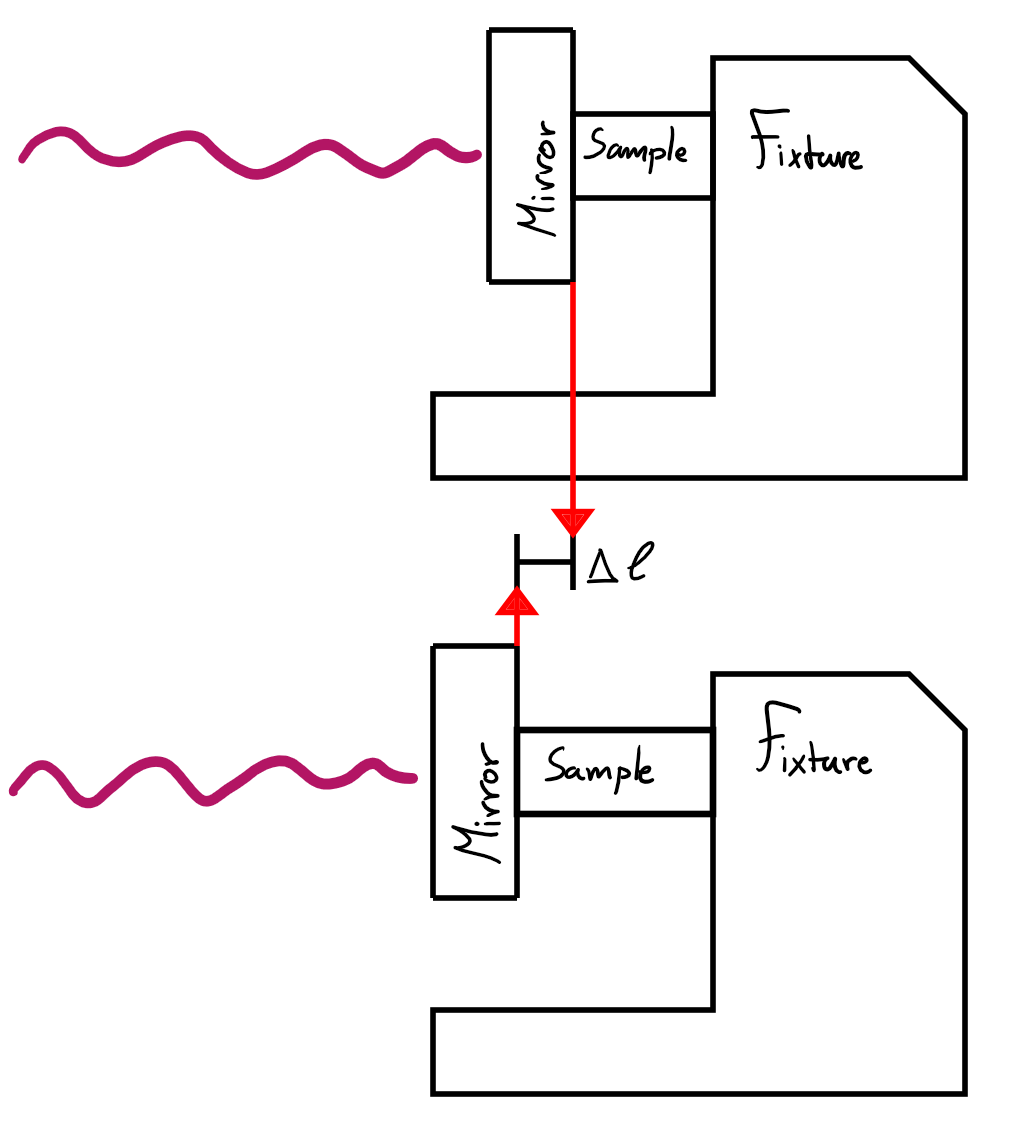
\includegraphics[width=0.9\linewidth]{./images/sample_mirror.png}

    % this determines where your columns will be separated
    \columnbreak

        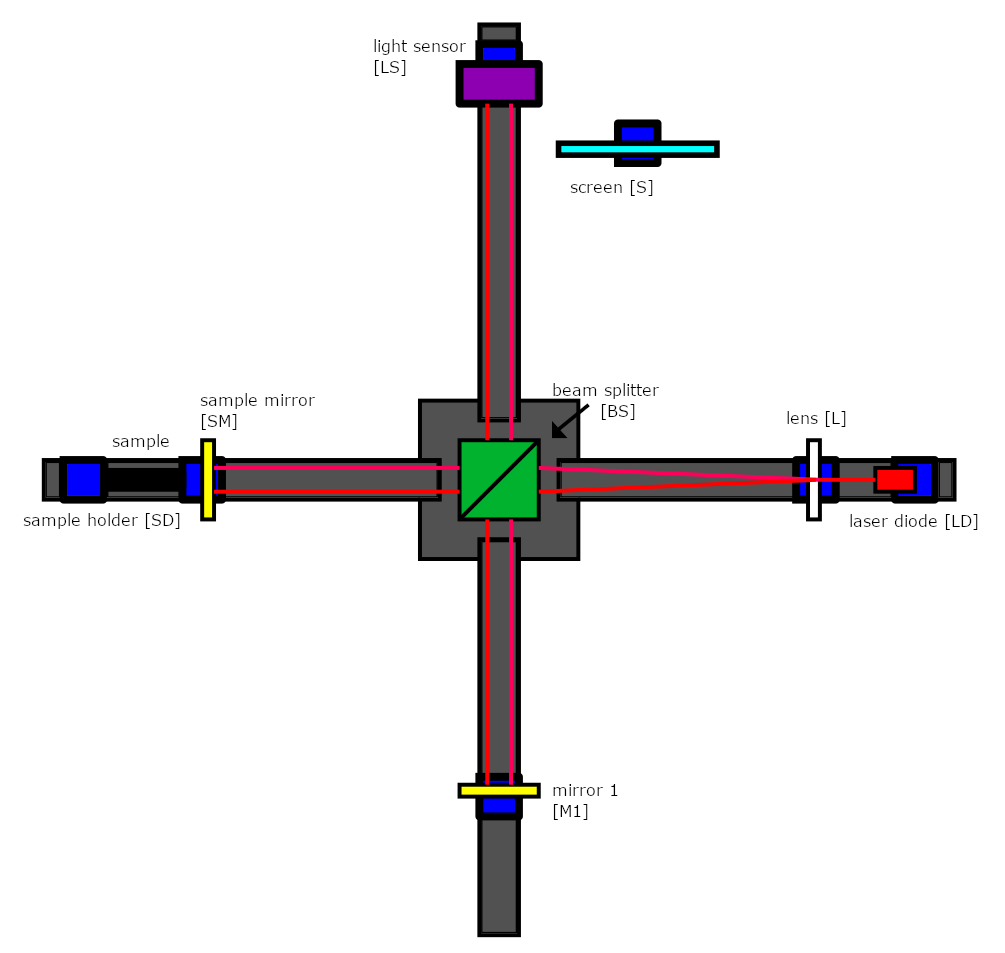
\includegraphics[width=1.1\linewidth]{./images/setup.png}

        \section{Results}
        \begin{itemize}
        \setlength\itemsep{0.1em}
            \item a
            \item b
            \item c
            \item d
            \item e
            \item f
        \end{itemize}

    \end{multicols}
}
% If you have extra figures or data to show
\makeextracolumn{

    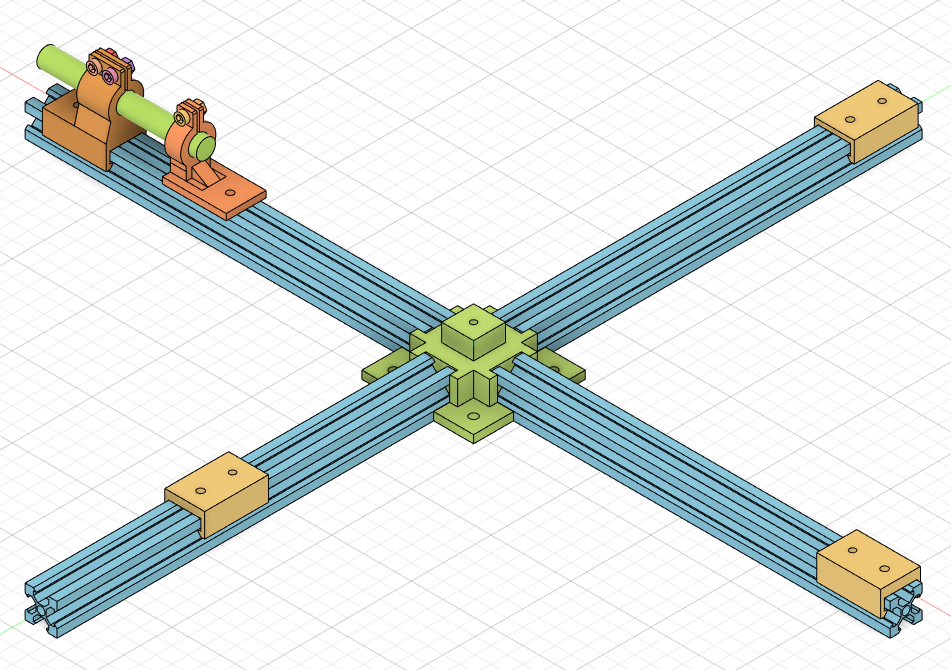
\includegraphics[width=0.9\linewidth]{./images/design.png}
    \linebreak
    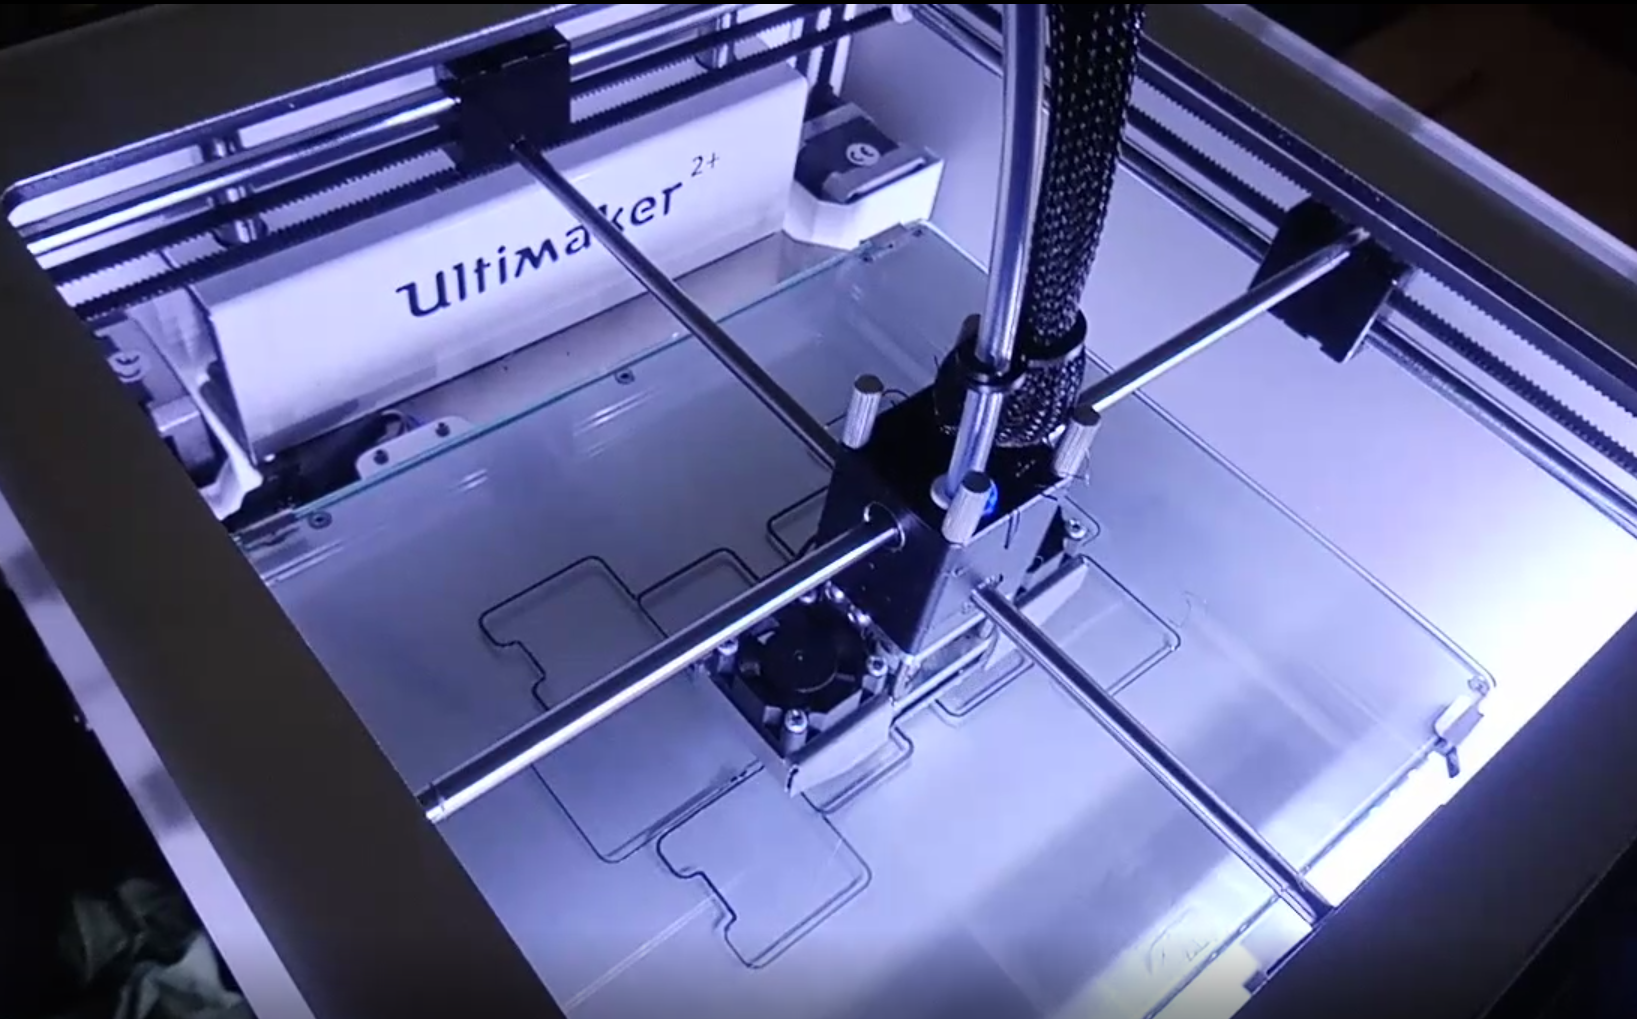
\includegraphics[width=0.9\linewidth]{./images/print.png}
    \linebreak
    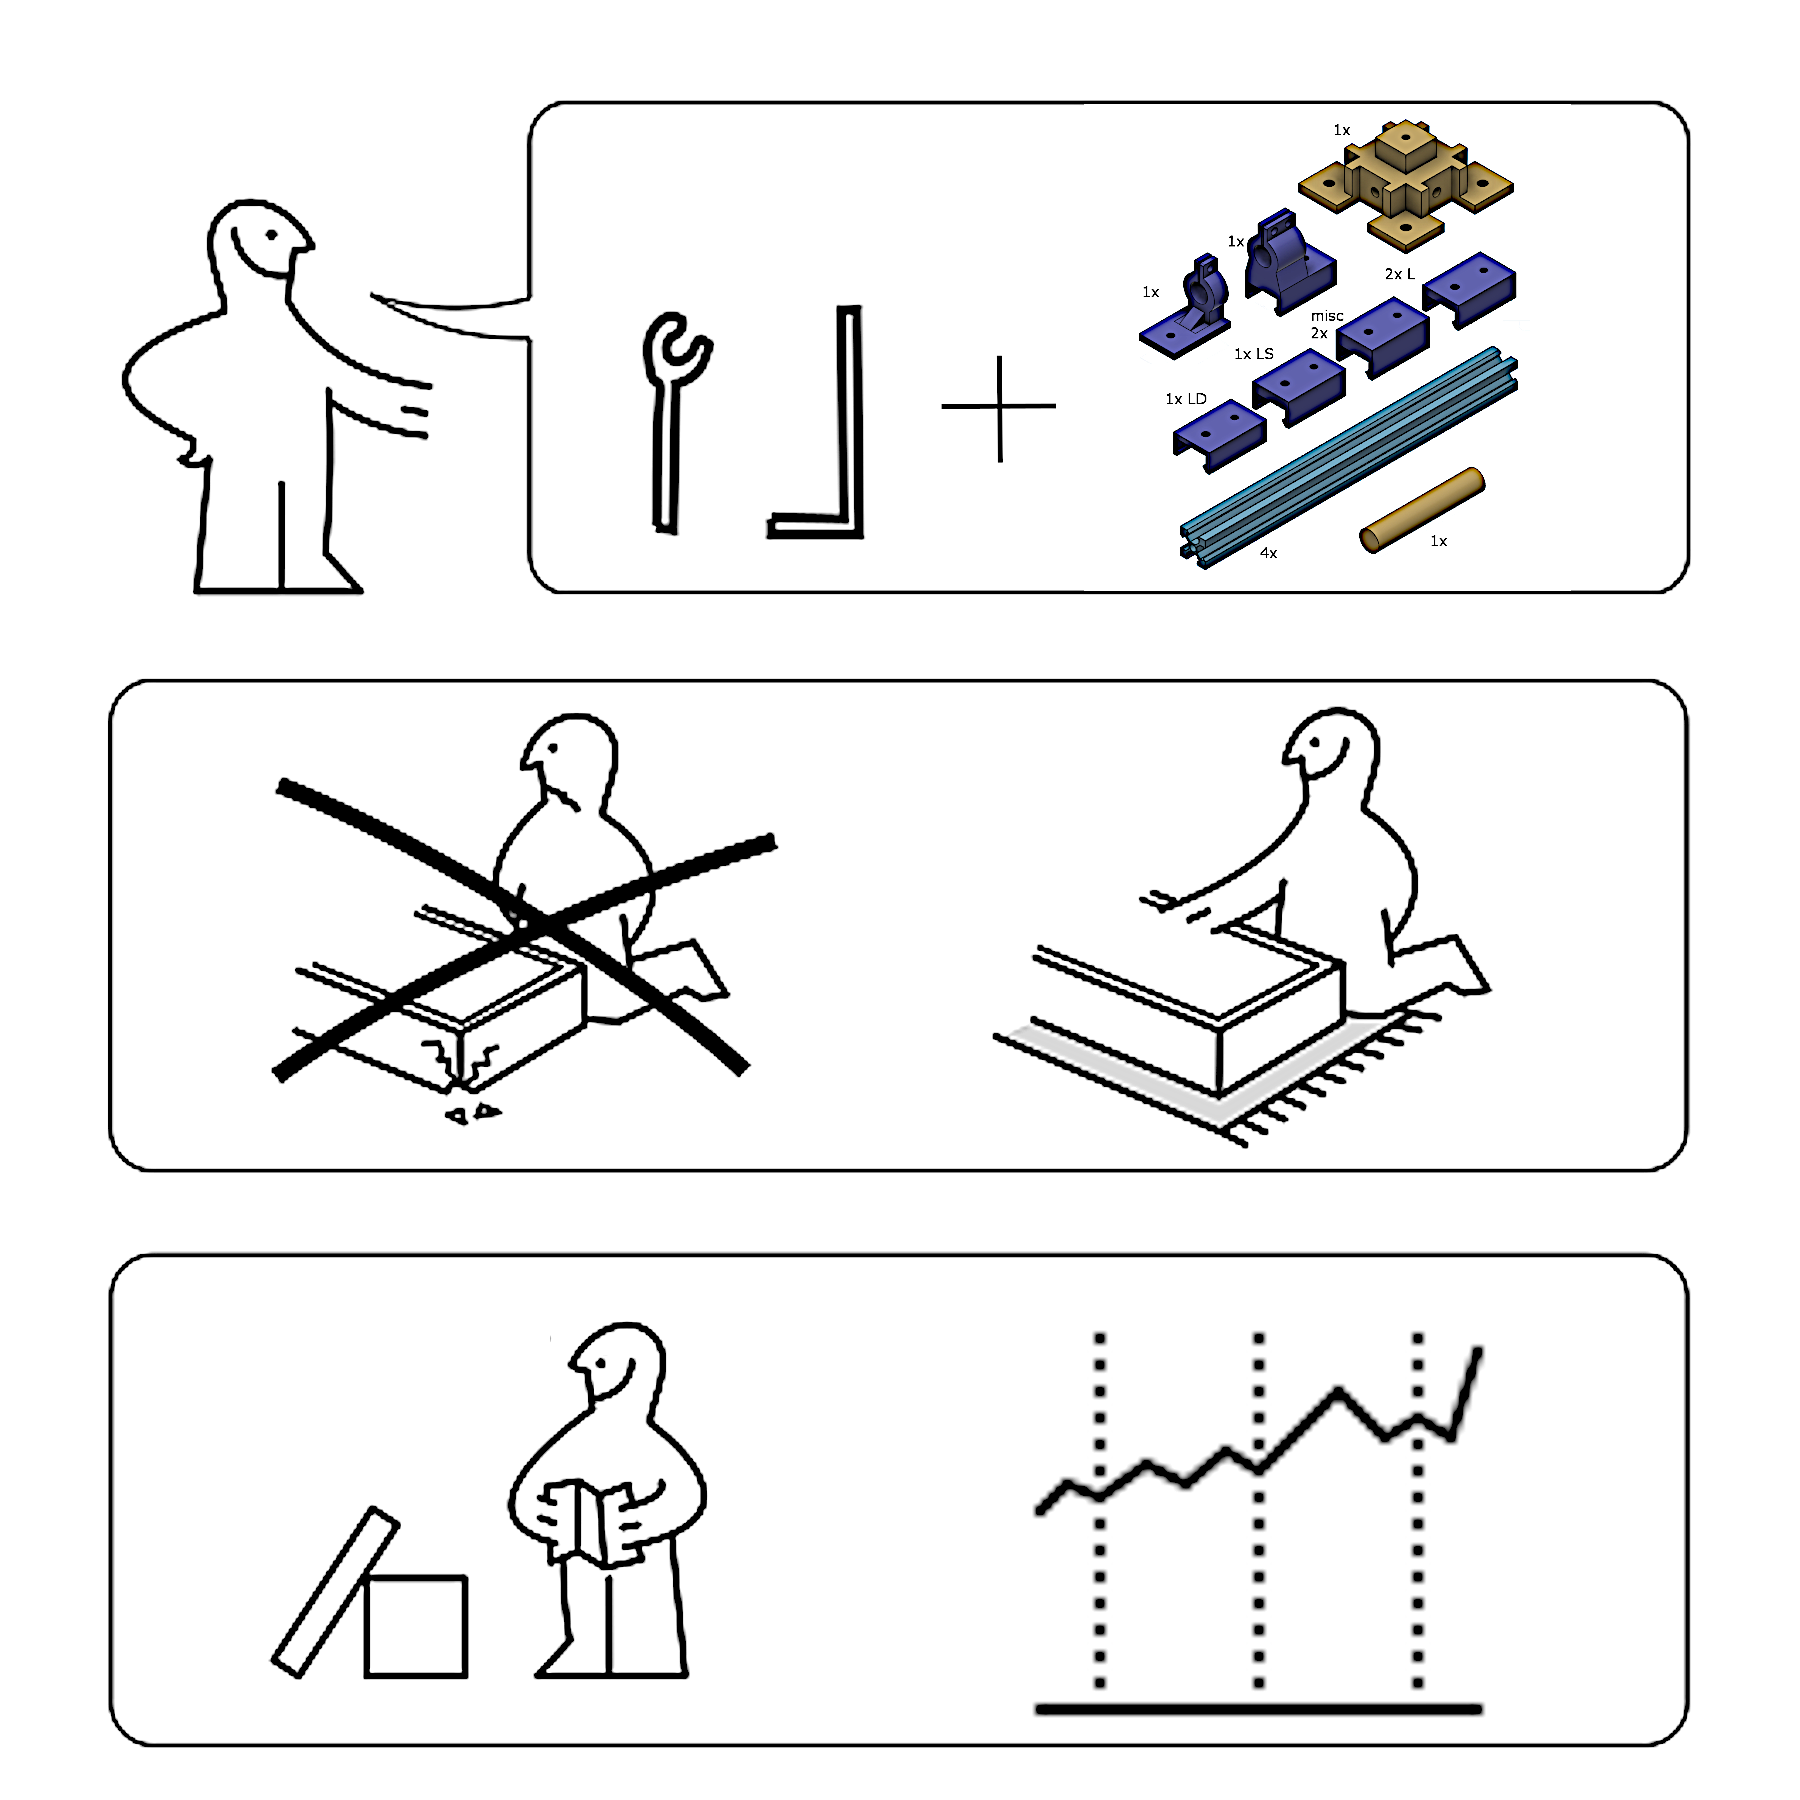
\includegraphics[width=0.9\linewidth]{./images/build.png}

}
% footer
% generate qr code from https://www.qr-code-generator.com/ and replace qr_code.png
% default: barcode on the left
\makefooter{images/uni_logo.png}{images/qr-code.png}

% replace with this like for barcode on the right
%\makealtfooter{images/uni_logo.png}{images/qr-code.png}

\end{document}
